\documentclass{article}

\usepackage{graphicx, xcolor}
\usepackage{amsmath, amssymb}
\usepackage{float}
\usepackage[colorlinks=true,allcolors=blue]{hyperref}

\usepackage[margin=1in]{geometry}

\def\hwtitle{Homework 8: Molecular dynamics}
\def\hwauthor{Caden Gobat}
\def\hwdate{\today}

\usepackage{fancyhdr}
\lhead{\hwauthor}
\chead{\hwtitle}
\rhead{\hwdate}
\lfoot{\hwauthor}
\cfoot{}
\rfoot{\thepage}
\renewcommand{\footrulewidth}{0.4pt}
\pagestyle{fancy}

\author{\hwauthor}
\title{\hwtitle}
\date{\hwdate}

\begin{document}

\maketitle
\thispagestyle{fancy}

\section{Introduction}

In this assignment, we return to $N$-body simulation to model a semi-ideal gas system of particles in a box, a field of computation known as molecular dynamics.

\section{Results}

\bigskip
\noindent{\bf Question 1}
\medskip

For the system with $E/N=-1.2$, the particles are all relatively clustered after thermalization, with only a few off on their own (Fig.~\ref{fig:1a}). In the system with $E/N=4$, however, we see the particles much more independently distributed, because they are able to break free of each others' potential wells (Fig.~\ref{fig:1b}). The first is what we might see for liquid water, with a few molecules having evaporated, but most stuck together. The second is more reminiscent of water vapor, where the molecules are mostly free-standing.

\begin{figure}[H]
    \centering
    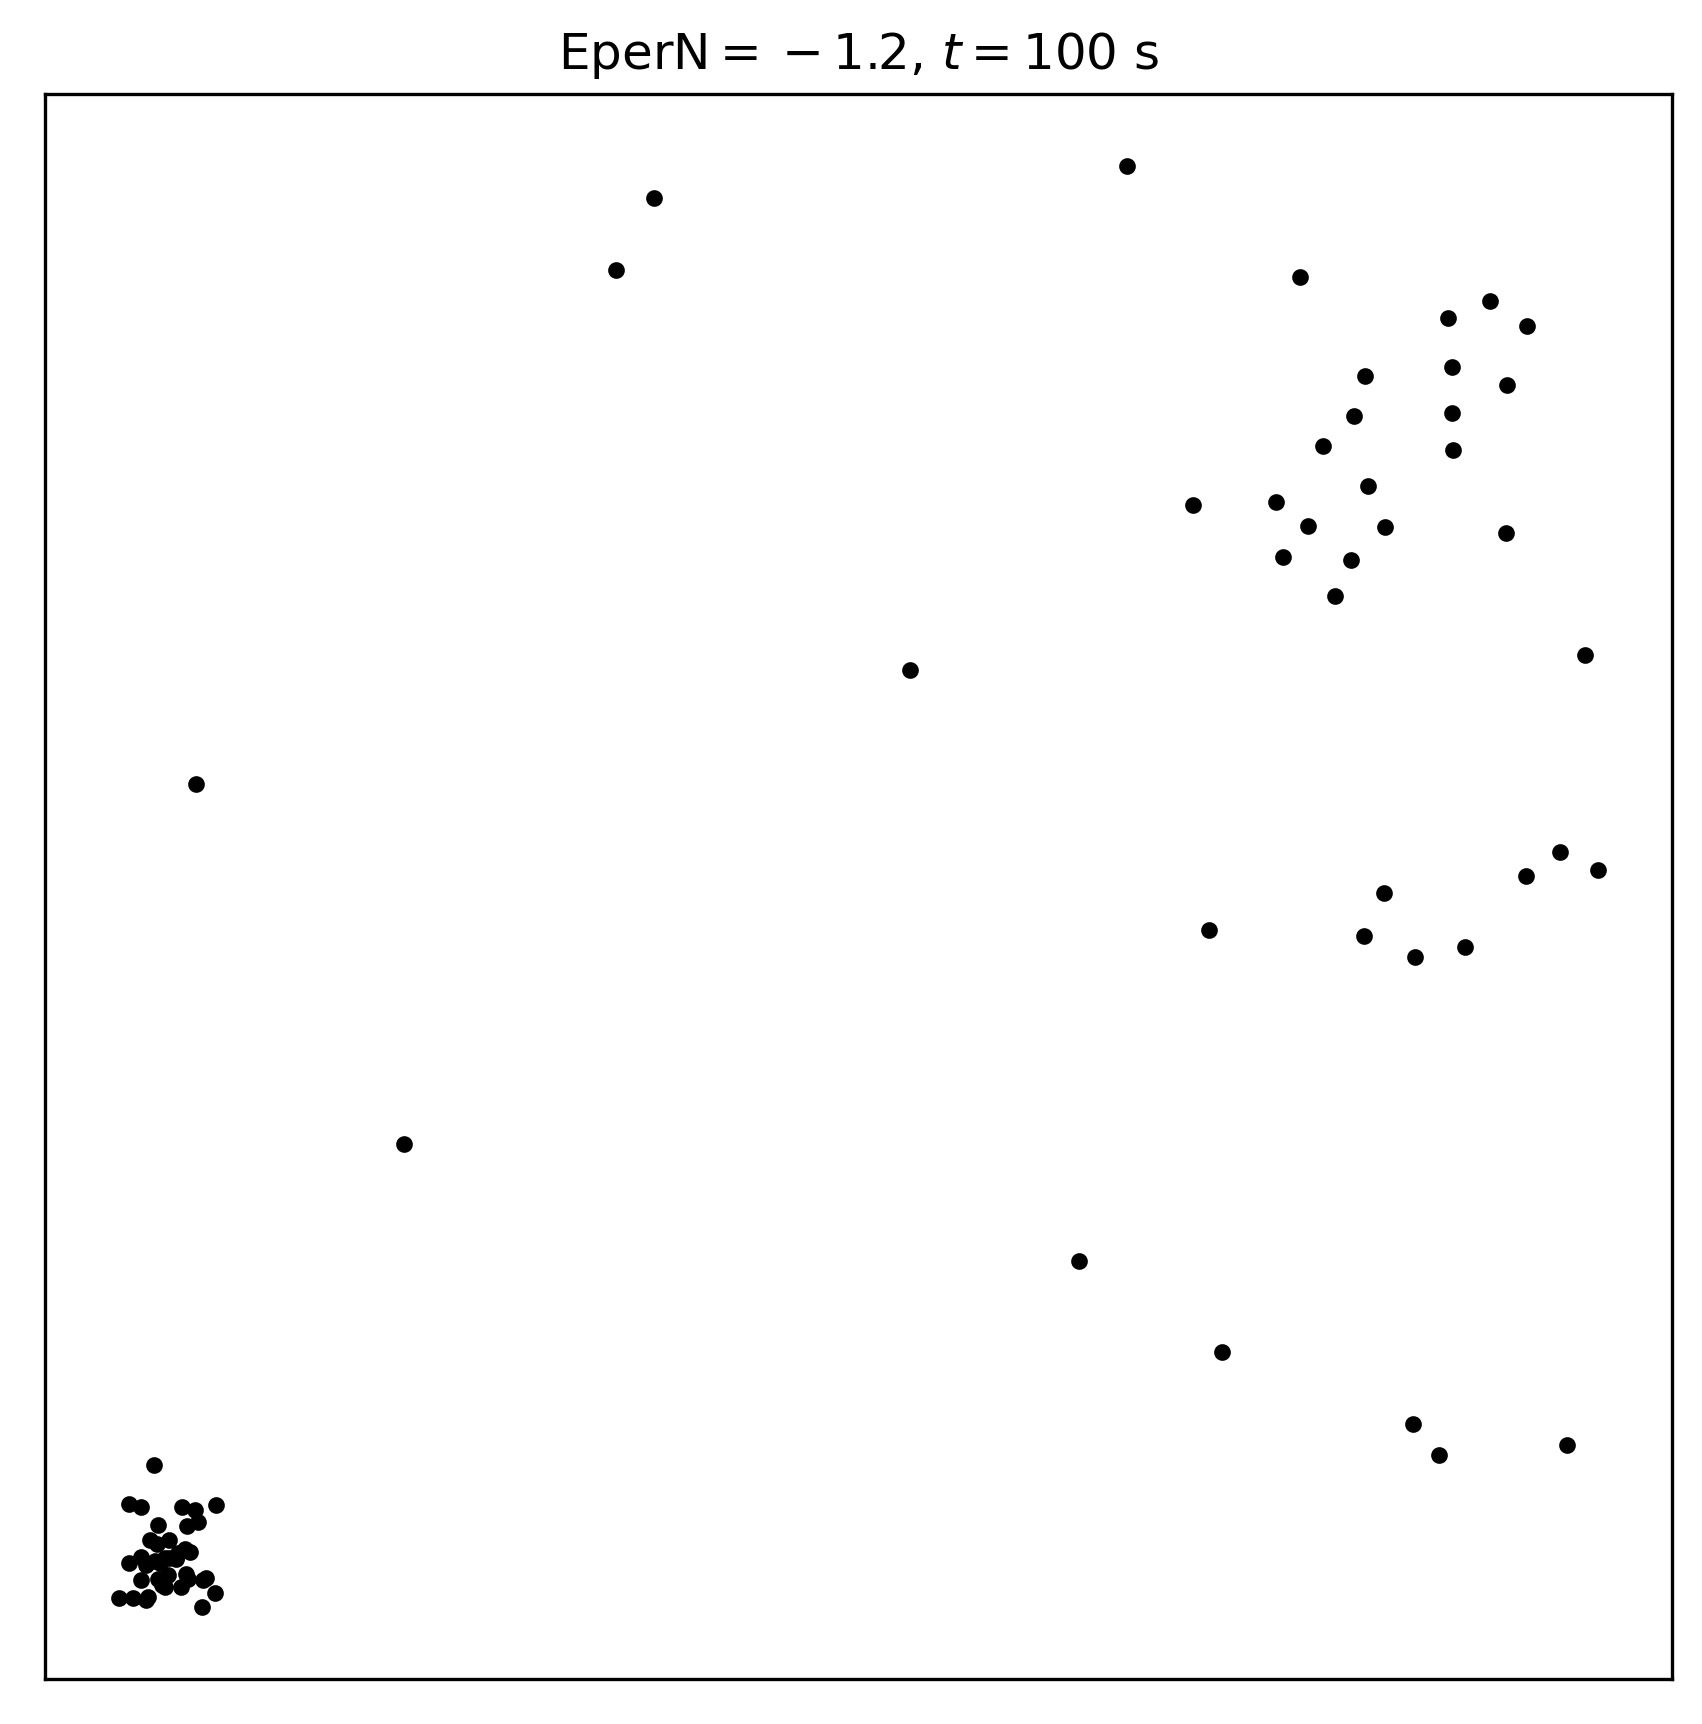
\includegraphics[width=4in]{homework8/p1a.png}
    \caption{$N=80$, $L=40$, $E/N=-1.2$, and $t=100$ s.}
    \label{fig:1a}
\end{figure}

\begin{figure}[H]
    \centering
    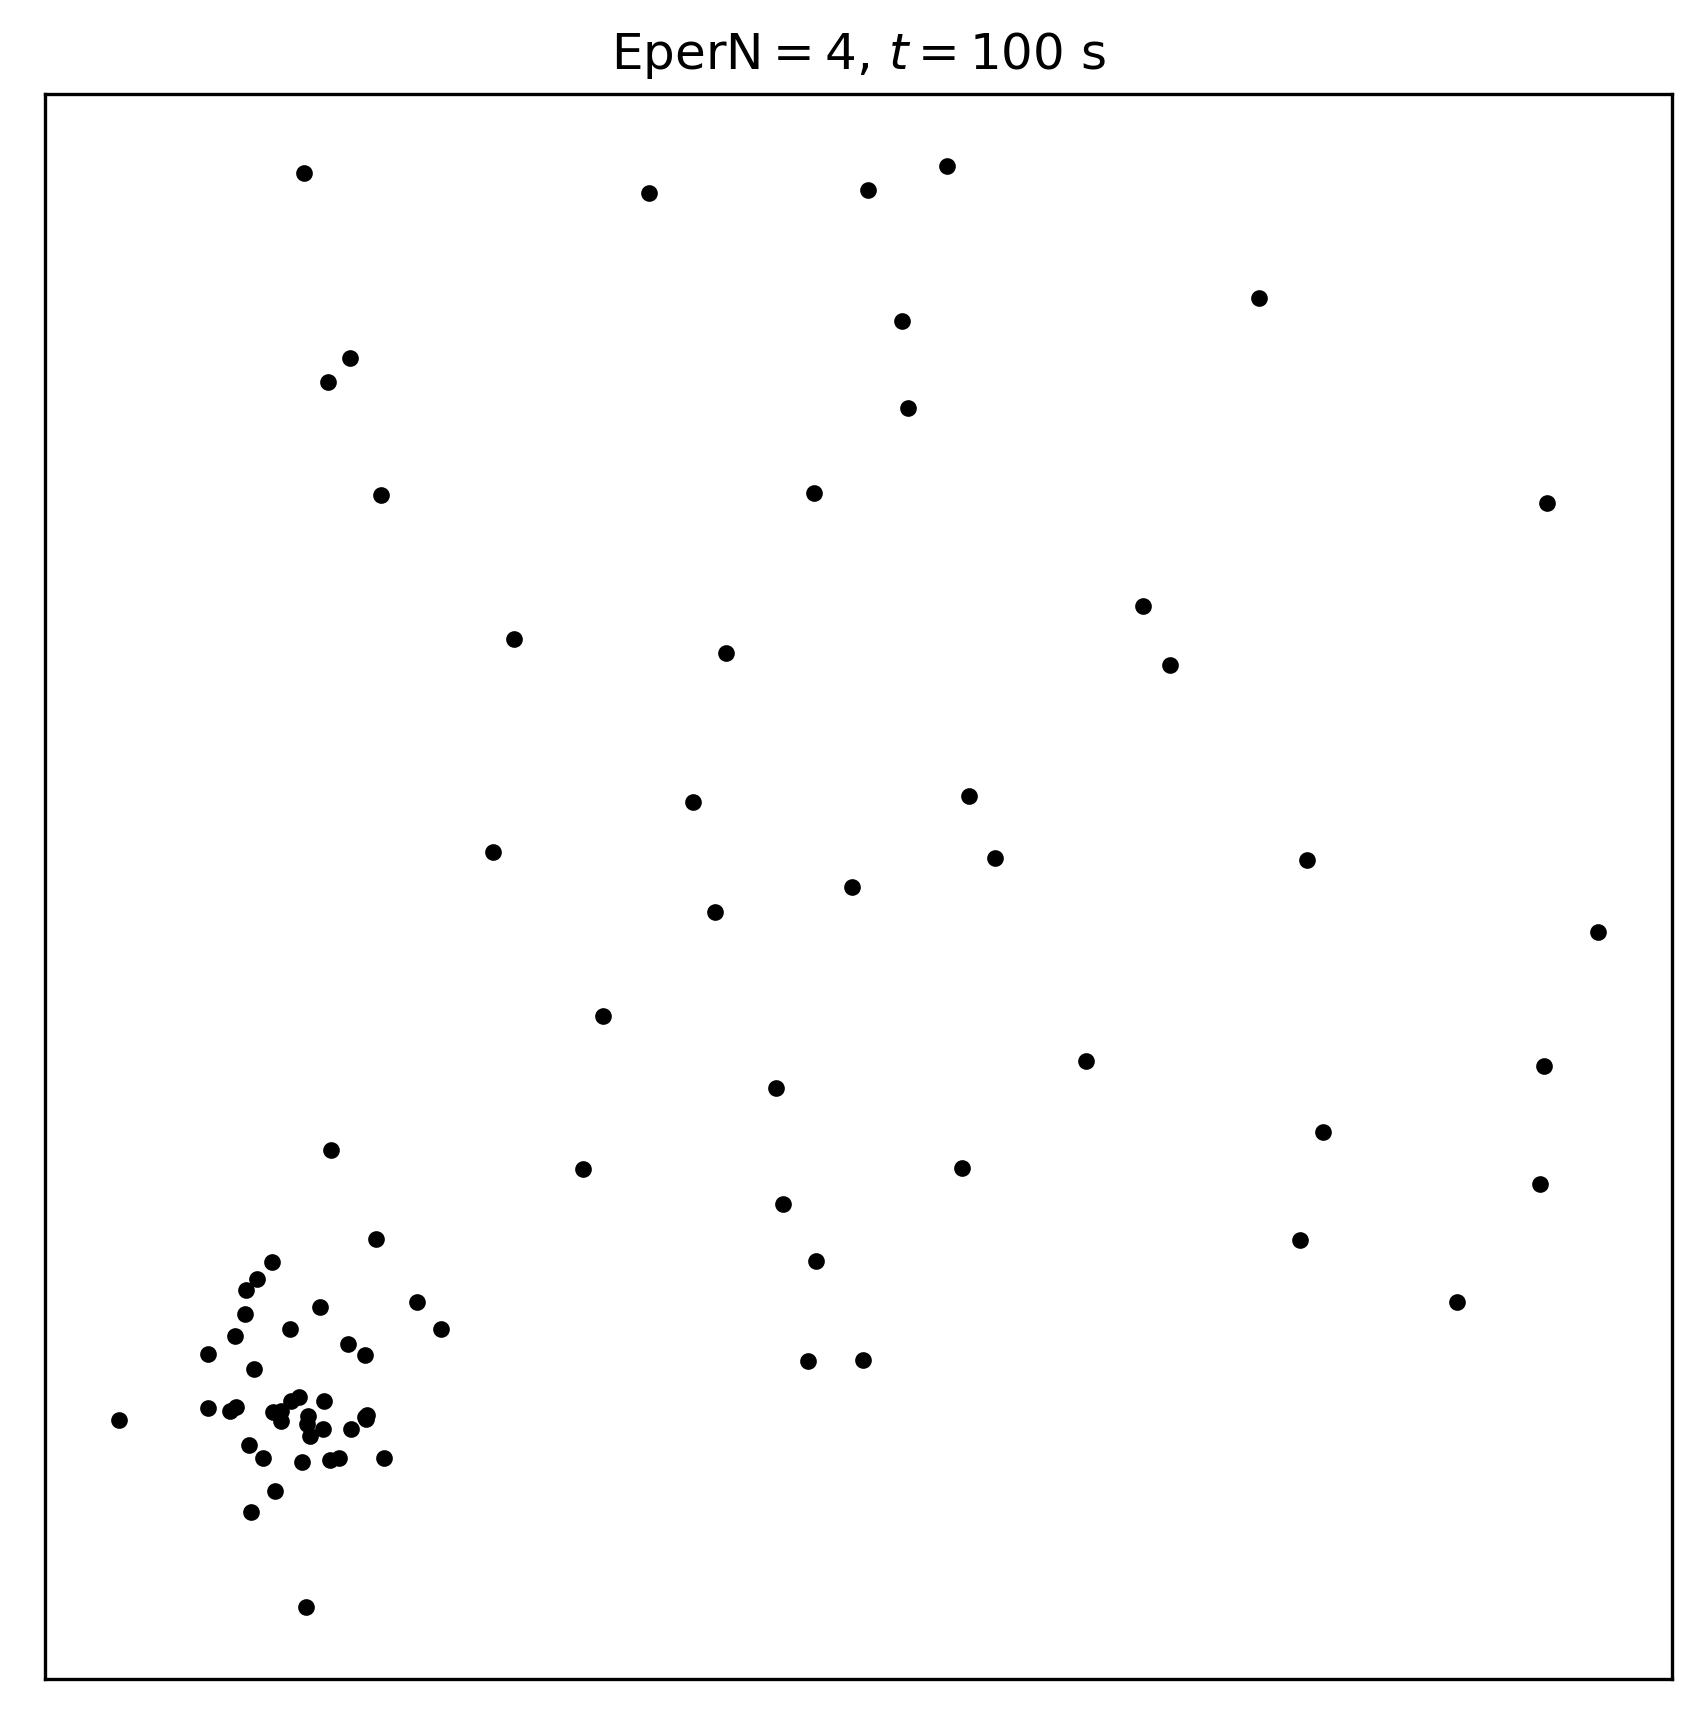
\includegraphics[width=4in]{homework8/p1b.png}
    \caption{$N=80$, $L=40$, $E/N=4$, and $t=100$ s.}
    \label{fig:1b}
\end{figure}

\bigskip
\noindent{\bf Question 2}
\medskip

\begin{figure}[H]
    \centering
    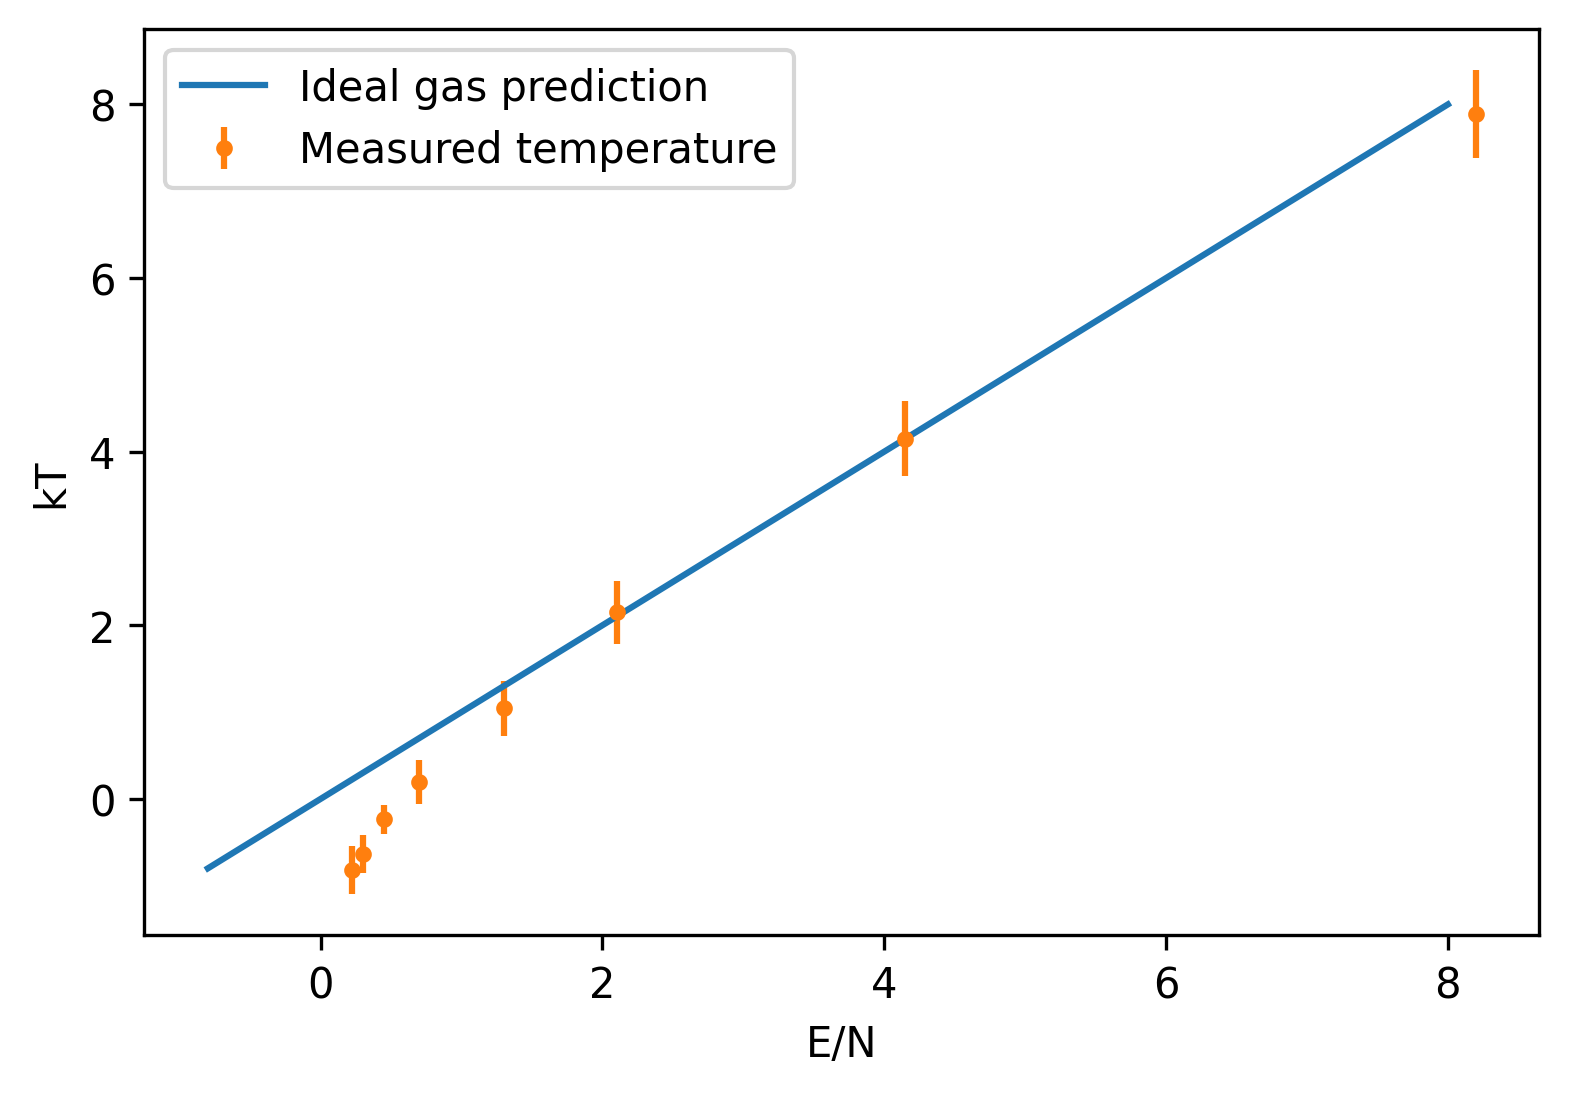
\includegraphics[width=4.75in]{homework8/p2a.png}
    \caption{Comparison of simulation ($N=20$, $L=40$, and $dt=10^{-3}$) temperature and ideal gas prediction as a function of $E\over N$. We see that the simulation is only really good for ${E\over N} > 0$.}
    \label{fig:2a}
\end{figure}

\begin{figure}[H]
    \centering
    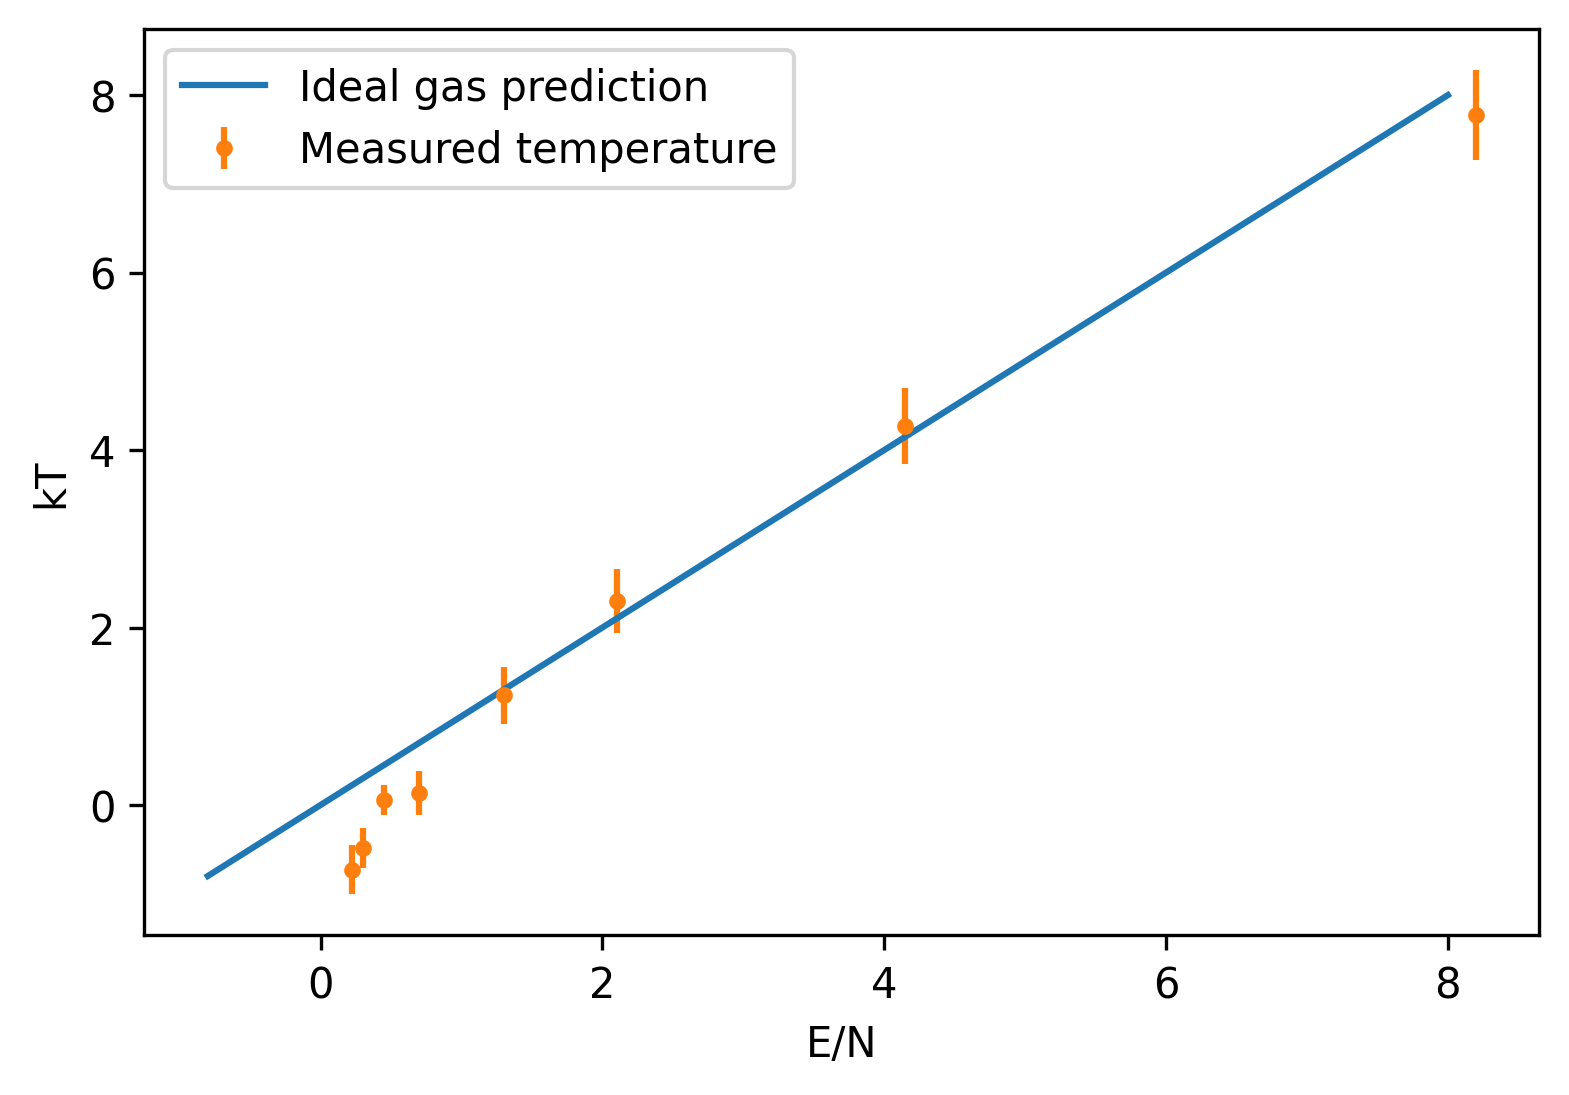
\includegraphics[width=4.75in]{homework8/p2b.png}
    \caption{Comparison of simulation ($N=20$, $L=16$, and $dt=10^{-3}$) temperature and ideal gas prediction as a function of $E\over N$. This plot is not qualitatively substantially different from Fig.~\ref{fig:2a}, so changing the dimensions (and therefore density) does not seem to significantly change the restriction of the simulation to ${E\over N}>0$.}
    \label{fig:2b}
\end{figure}

\bigskip
\noindent{\bf Question 3}
\medskip

The velocity distributions for each scenario are shown in Fig.\ref{fig:3a} and Fig.~\ref{fig:3b}, respectively.

\begin{figure}[H]
    \centering
    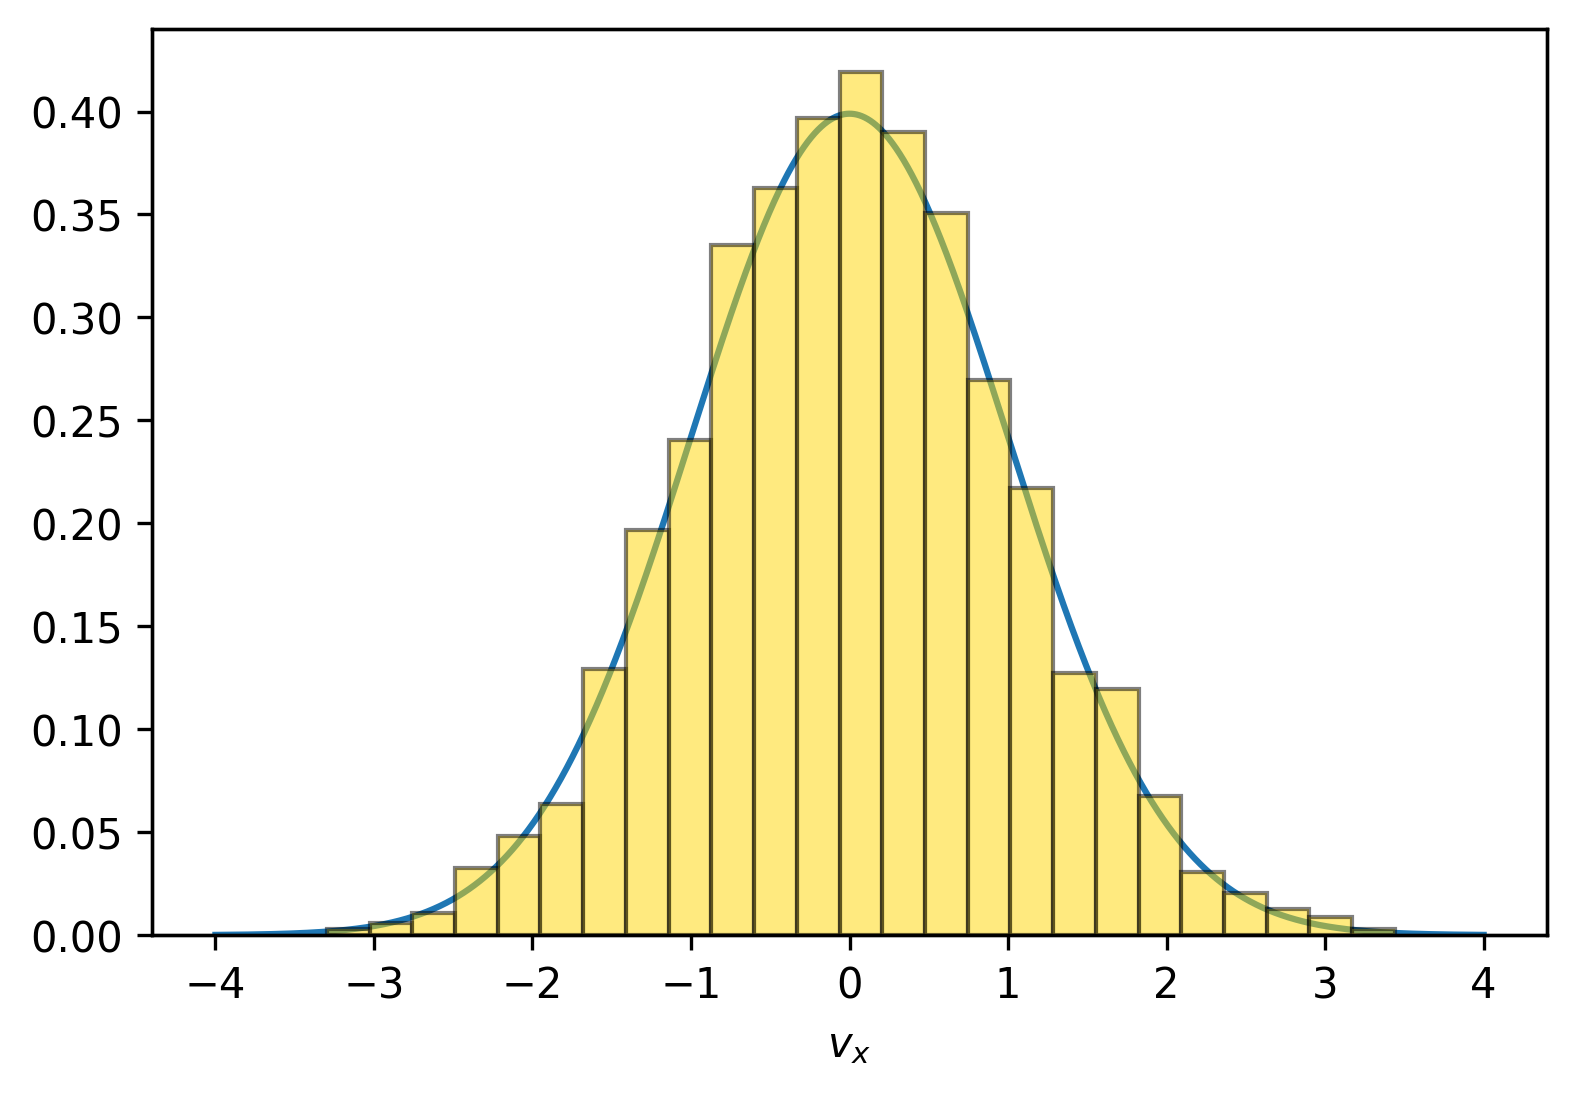
\includegraphics[width=4.75in]{homework8/p3a.png}
    \caption{Distribution of $x$-velocities when $N=40$, $L=40$, and $E/N=1.2$. We observe a close agreement between the simulation histogram (in gold) and the theoretical Maxwell-Boltzmann distribution (in blue).}
    \label{fig:3a}
\end{figure}

\begin{figure}[H]
    \centering
    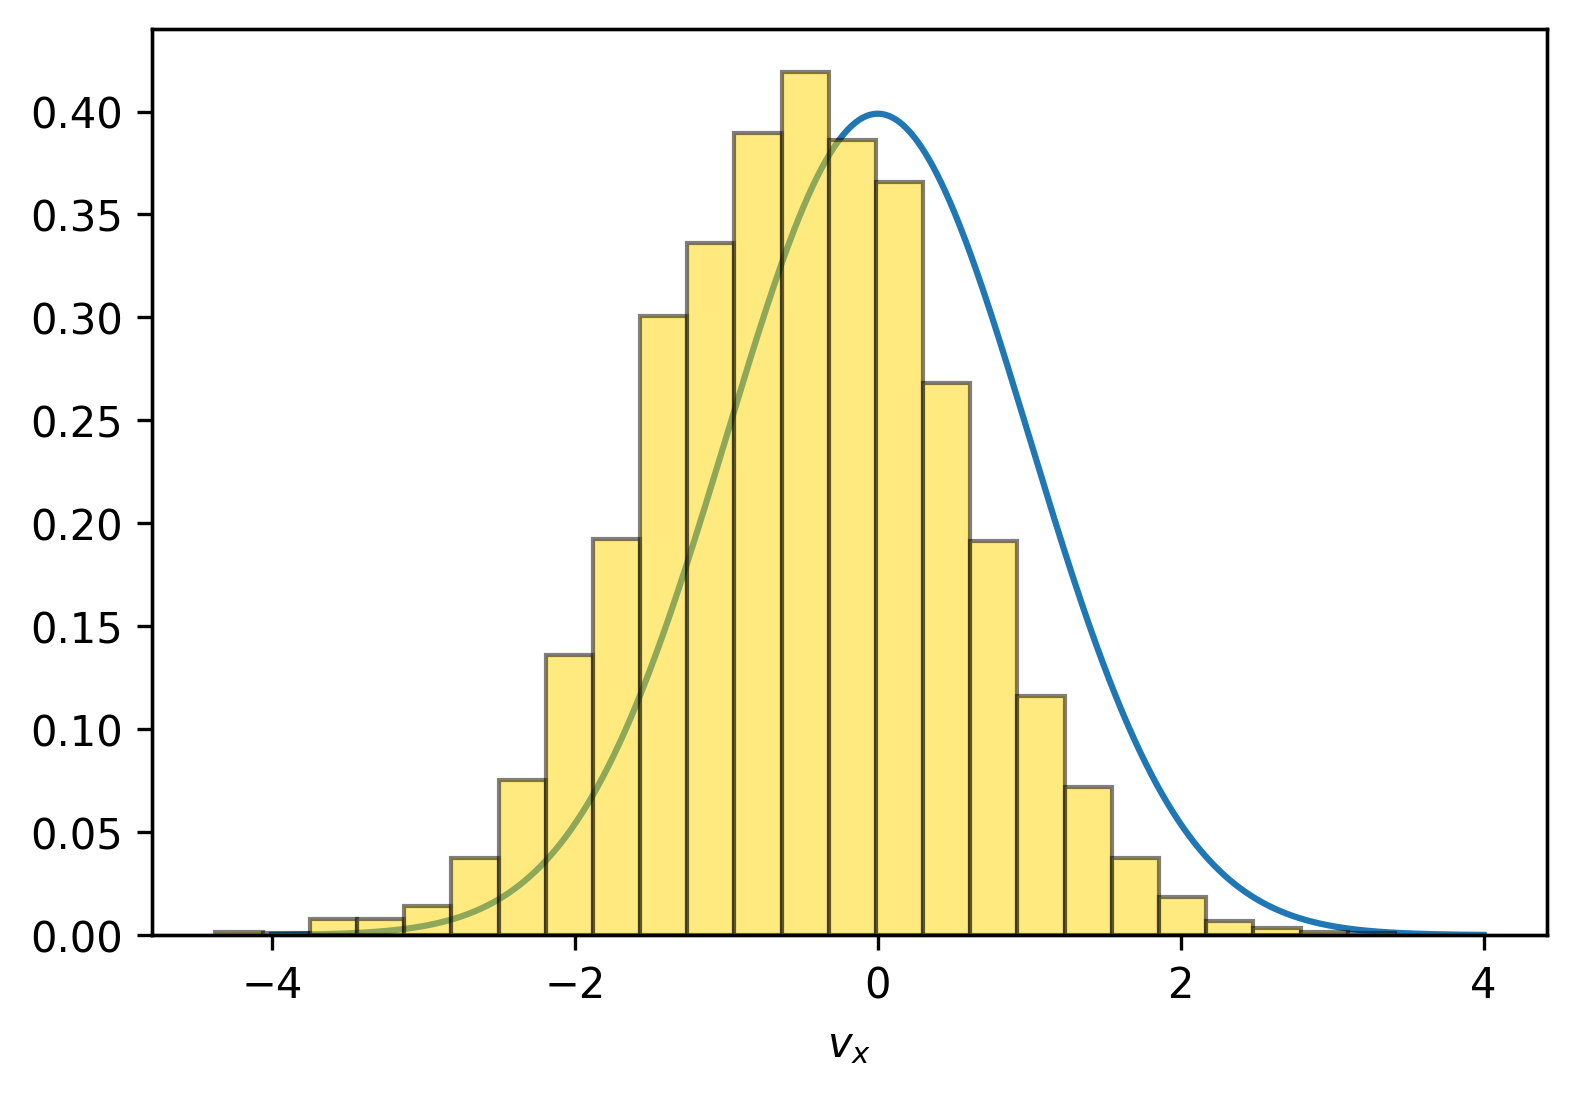
\includegraphics[width=4.75in]{homework8/p3b.png}
    \caption{Distribution of $x$-velocities when $N=40$, $L=40$, and $E/N=-0.8$. We observe a slight skew between the simulation histogram (in gold) and the theoretical Maxwell-Boltzmann distribution (in blue), which could be attributed to some kind of overall motion of the group of particles.}
    \label{fig:3b}
\end{figure}

\bigskip
\noindent{\bf Question 4}
\medskip

\begin{figure}[H]
    \centering
    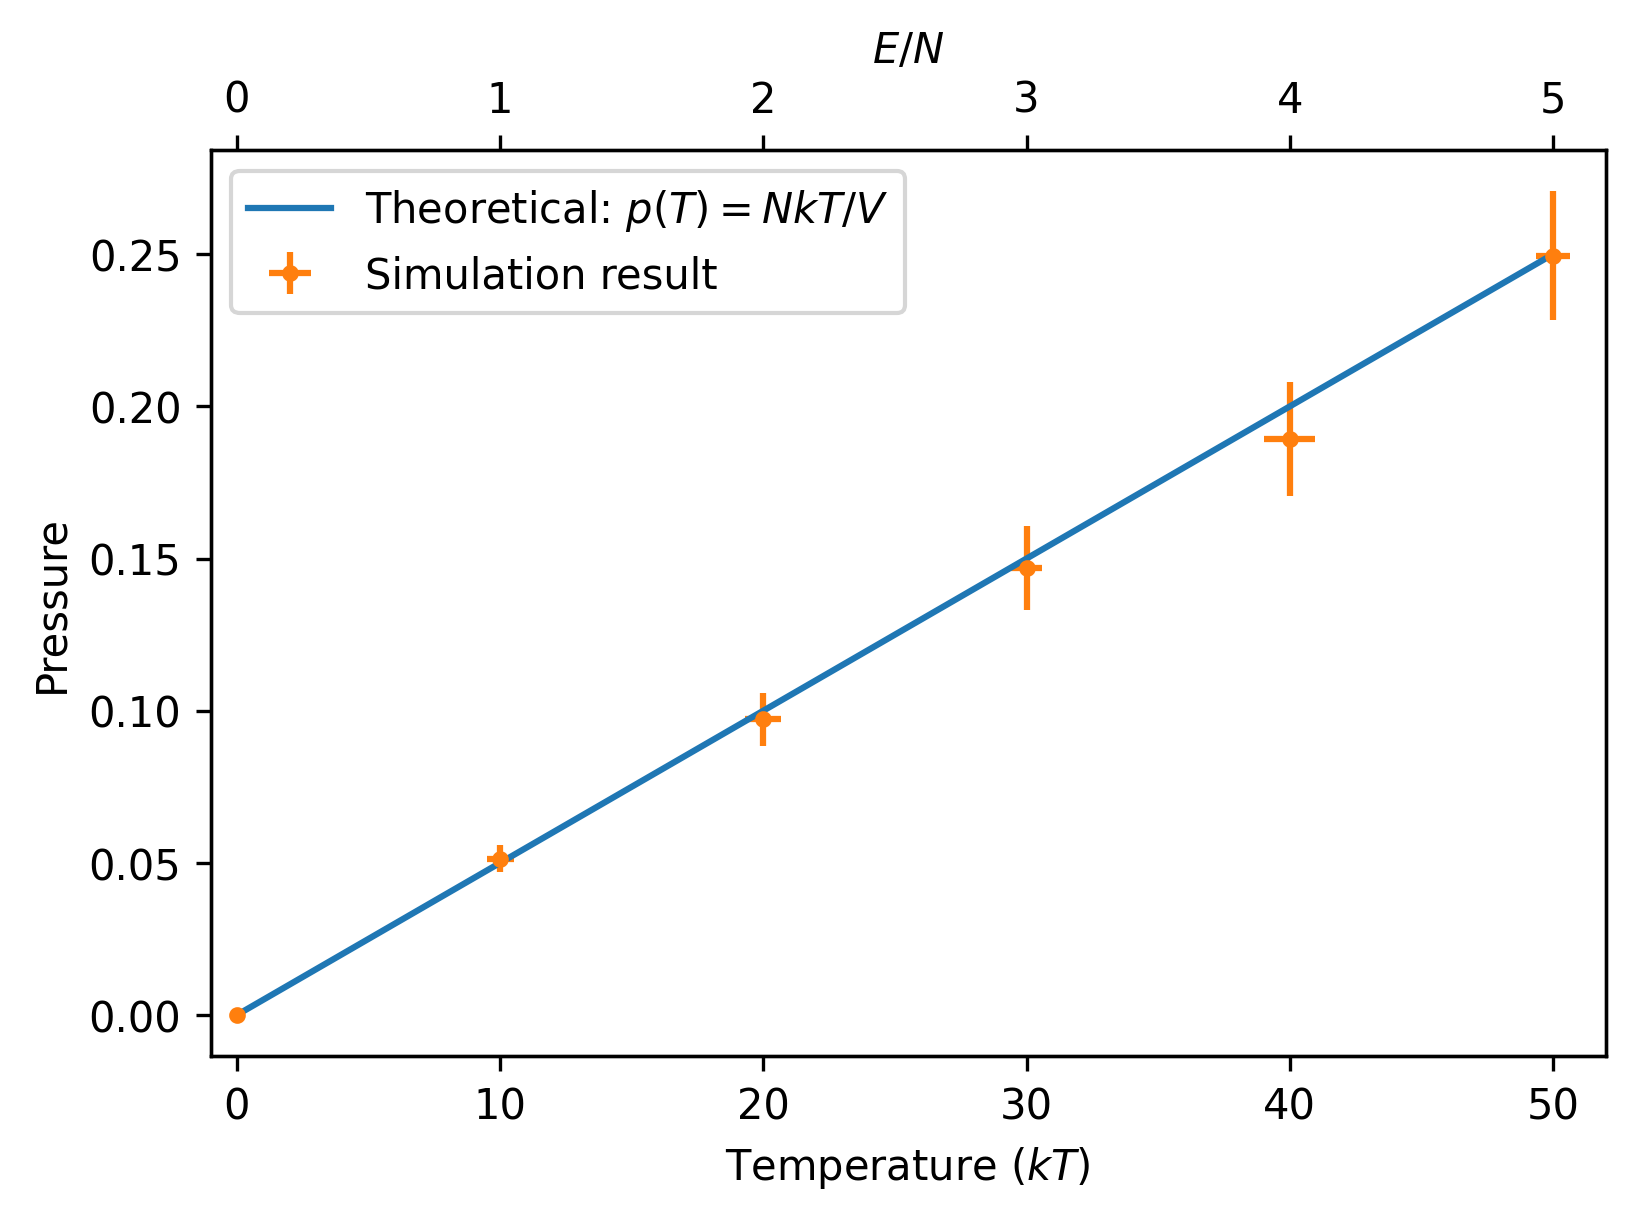
\includegraphics[width=4.75in]{homework8/p4.png}
    \caption{Comparison of simulation results (blue) and theoretical ideal gas formula for pressure (orange). In general we observe a reasonable degree of agreement between the two.}
    \label{fig:4}
\end{figure}

\section{Conclusions}

This assignment was a bit challenging, and the fact that my computer took quite a while to run each simulation with $dt=10^{-3}$ was a bit of an obstacle, but in the end I learned quite a lot about the principles of molecular dynamics. I was especially interested in this topic because it is closely related to the material I am studying concurrently in another class, Thermal \& Statistical Physics.

\end{document}